
\documentclass[letterpaper, reqno,11pt]{article}
\usepackage[margin=1.0in]{geometry}
\usepackage{color,latexsym,amsmath,amssymb}
\usepackage{fancyhdr}
\usepackage{amsthm}
\usepackage{mathtools}
\usepackage{tikz}
\usepackage{float}
\usepackage{centernot}
\usepackage{subcaption}
\usepackage{extarrows}
\usetikzlibrary{hobby}
\usetikzlibrary{shapes.multipart}
\usepackage{pgfplots}
\pgfplotsset{compat=1.7}

\newcommand{\RR}{\mathbb{R}}
\newcommand{\CC}{\mathbb{C}}
\newcommand{\ZZ}{\mathbb{Z}}
\newcommand{\QQ}{\mathbb{Q}}
\newcommand{\NN}{\mathbb{N}}
\DeclareMathOperator{\card}{card}
\DeclareMathOperator{\Binomial}{Binomial}
\pagestyle{fancy}
\lhead{Math 321 Lecture 10}
\rhead{Yuchong Pan}
\begin{document}
\pagenumbering{arabic}
\title{Math 321 Lecture 10}
\author{Yuchong Pan}
\date{January 23, 2019}
\newtheorem{thm}{Theorem}
\newtheorem{defn}{Definition}
\newtheorem*{remark}{Remark}
\newtheorem{claim}{Claim}
\newtheorem{cor}{Corollary}
\newtheorem{lemma}{Lemma}
\newtheorem{prop}{Proposition}
\maketitle
%

\section{Stone-Weierstrass Theorem (Cont'd)}

\begin{thm}[Stone-Weierstrass theorem]
  \normalfont Let $(X, d)$ be a compact metric space. Let $\mathcal A \subseteq \underbrace{C(X; \RR)}_\text{all continuous functions from $X$ to $\RR$}$ be a {\bf sub-algebra} that {\bf separates points} and {\bf vanishes at no point}. Then $\mathcal A$ is dense in $C(X; \RR)$; i.e., $\overline{\mathcal A} = C(X; \RR)$.
\end{thm}

\noindent\fbox{\begin{minipage}{\textwidth}
    \begin{lemma} \label{lem:1}
      \normalfont Suppose $\mathcal A$ be any algebra of real-valued functions that separates points and vanishes at no point. Then given any $\underbrace{x_0, y_0 \in X}_{x_0 \neq y_0}$ and $a, b \in \RR$, there exists $F \in \mathcal A$ such that $F(x_0) = a$ and $F(y_0) = b$.
    \end{lemma}
\end{minipage}}

\noindent Compactness of $X$ is not needed. Further, continuity of functions in $\mathcal A$ are not assumed.

~

\noindent\fbox{\begin{minipage}{\textwidth}
    \begin{prop} \label{prop:1}
      \normalfont Let $\mathcal A \subseteq C(X; \RR)$ be a sub-algebra. Then $\overline{\mathcal A}$ is also a sub-algebra and a {\bf sub-lattice}; i.e., $\fbox{if $F \in \mathcal A$, then $|F| \in \mathcal A$}$.
    \end{prop}
\end{minipage}}

\qquad \qquad \qquad \qquad \quad $\Downarrow$

\noindent For any two functions $F_1$ and $F_2$ in $\mathcal A$, their maximum $F = \max(F_1, F_2) \in \mathcal A$.

\noindent The analogous statement holds for the minimum of two functions.

\begin{figure}[H]
  \centering
  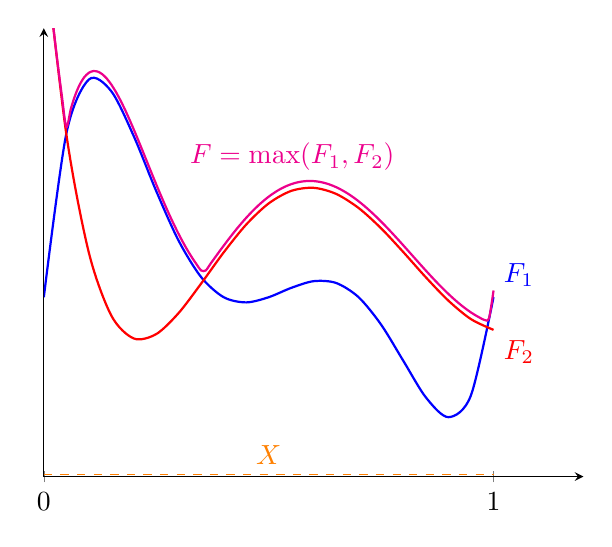
\begin{tikzpicture}[
      declare function={f1(\x)=-0.75*\x*(\x-0.4)*(\x-0.5)*(\x-0.7)*(\x-1)*(\x-100)+0.4;},
      declare function={f2(\x)=-10*(\x-0.1)*(\x-0.4)*(\x-0.8)*(\x-1.2)*(\x-1.8)+0.5;},
      declare function={f(\x)=max(f1(\x), f2(\x));},
    ]
    \begin{axis}[
        xmin=0,
        xmax=1.2,
        ymin=0,
        ymax=1,
        xtick={0, 1},
        xticklabels={$0$, $1$},
        ymajorticks=false,
        axis x line=bottom,
        axis y line=left,
      ]
      \addplot[thick, blue, samples at={0,0.05,...,1}, smooth](x,{f1(x)}) node [above right] {$F_1$};
      \addplot[thick, red, samples at={0,0.05,...,1}, smooth](x,{f2(x)}) node [below right] {$F_2$};
      \addplot[thick, magenta, samples at={0,0.01,...,1}, smooth](x,{f(x)+0.015}) node [midway, above right, yshift=0.7cm] {$F = \max(F_1, F_2)$};
      \draw[dashed, orange] (axis cs:0,0.005) -- (axis cs:1,0.005) node [midway, above] {$X$};
    \end{axis}
  \end{tikzpicture}
\end{figure}

\noindent {\bf Note:} $|G| = \max(G, -G)$ for any real $G$. Thus,
\begin{align*}
  |F_1 - F_2| &= \max(F_1 - F_2, F_2 - F_1), \\
  \frac{1}{2}(F_1 + F_2 + |F_1 - F_2|) &= \left\{
  \begin{array}{ll}
    \frac{1}{2} (F_1 + F_2 + F_1 - F_2) = F_1, & F_1 \geq F_2, \\
    \frac{1}{2} (F_1 + F_2 + F_2 - F_1) = F_2, & F_1 < F_2,
  \end{array}
  \right. = \max(F_1, F_2).
\end{align*}

\begin{proof}[Proof of SW assuming Lemma \ref{lem:1} and Proposition \ref{prop:1}]
  \renewcommand{\qedsymbol}{}
  Start with $f \in C(X; \RR)$ and fix $\epsilon > 0$. We wish to find $g \in \mathcal A$ such that $\lVert f - g \rVert_\infty = \sup_{x \in X} |f(x) - g(x)| < \epsilon$.

  \noindent {\bf Step 1:} For every $x \in X$, we will find $g_x \in \mathcal A$ such that $g_x(x) = f(x)$ and that $g_x(y) > f(y) - \epsilon$ for all $y \in X$.

  \begin{figure}[H]
    \centering
    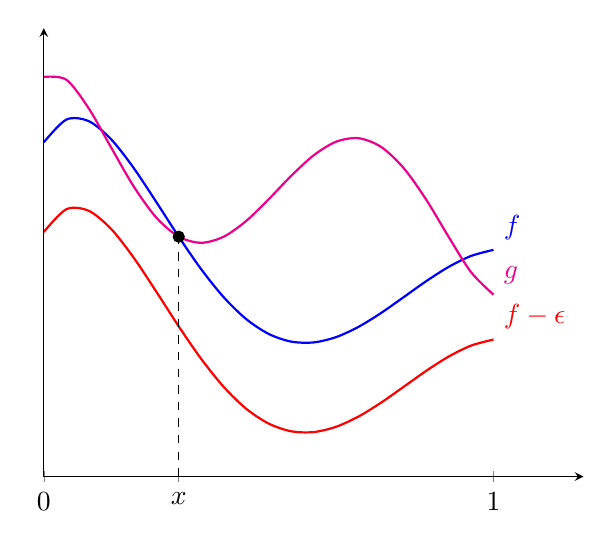
\begin{tikzpicture}[
        declare function={f(\x)=5*(\x+0.1)*(\x-0.4)*(\x-0.8)*(\x-1.2)*(\x-1.8)+0.4;},
        declare function={g(\x)=-2*(\x+0.1)*(\x-0.3)*(\x-0.4)*(\x-0.9)*(\x-1.1)*(\x-15)+0.535;},
      ]
      \begin{axis}[
          xmin=0,
          xmax=1.2,
          ymin=0,
          ymax=1,
          xtick={0, 0.3, 1},
          xticklabels={$0$, $x$, $1$},
          ymajorticks=false,
          axis x line=bottom,
          axis y line=left,
        ]
        \addplot[thick, blue, samples at={0,0.05,...,1}, smooth](x,{f(x)}) node [above right] {$f$};
        \addplot[thick, red, samples at={0,0.05,...,1}, smooth](x,{f(x)-0.2}) node [above right] {$f - \epsilon$};
        \addplot[thick, magenta, samples at={0,0.05,...,1}, smooth](x,{g(x)}) node [above right] {$g$};
        \draw[fill=black] (axis cs:0.3,{f(0.3)}) circle (2pt);
        \draw[dashed] (axis cs:0.3,0) -- (axis cs:0.3,{f(0.3)});
      \end{axis}
    \end{tikzpicture}
  \end{figure}

  \noindent {\bf Proof of Step 1:} For any $x \in X$, for every $y \neq x$, invoke Lemma \ref{lem:1} to find $G_y \in \mathcal A \subseteq C(X; \RR)$ such that
  \begin{equation} \label{eq:star} \tag{*}
    G_y(x) = f(x), \qquad G_y(y) = f(y).
  \end{equation}
  Note that $G_y - f \in C(X; \RR)$; hence its pre-images of open sets are open. This implies that
  $$ U_y = (G_y - f)^{-1} (-\epsilon, \infty) = \{ z \in X : (G_y - f)(z) > -\epsilon \} = \{ z \in X : G_y(z) > f(z) - \epsilon \} $$
  is oepn and contains $x$ and $y$.

  Hence, $\{ U_y ; y \in X, y \neq x \}$ forms an open cover of $X$. Since $X$ is compact, there is a finite subcover $U_{y_1}, U_{y_2}, \ldots, U_{y_M}$. Consider $g_x = \max(G_{y_1}, G_{y_2}, \ldots, G_{y_M})$. Since $X \subseteq U_{y_1} \cup U_{y_2} \cup \ldots \cup U_{y_M}$, then for every $y \in X$, there exists $j$ such that
  $$ y \in U_{y_j} \Rightarrow G_{y_j}(y) - f(y) > \epsilon \Rightarrow G_{y_j}(y) > f(y) - \epsilon. $$

  \begin{figure}[H]
    \centering
    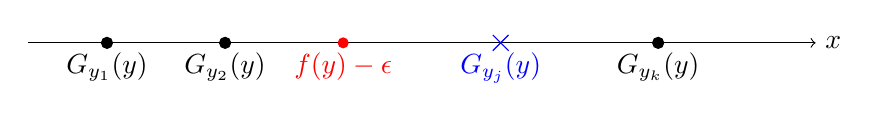
\begin{tikzpicture}
      \draw[->] (0, 0) -- (10, 0) node[right] {$x$};
      \draw[blue] (5.9, -0.1) -- (6.1, 0.1);
      \draw[blue] (5.9, 0.1) -- (6.1, -0.1);
      \node[below, blue] at (6, 0) {$G_{y_j}(y)$};
      \fill[red] (4, 0) circle (2pt);
      \node[below, red] at (4, 0) {$f(y) - \epsilon$};
      \draw[fill=black] (1, 0) circle (2pt) node[below] {$G_{y_1}(y)$};
      \draw[fill=black] (2.5, 0) circle (2pt) node[below] {$G_{y_2}(y)$};
      \draw[fill=black] (8, 0) circle (2pt) node[below] {$G_{y_k}(y)$};
    \end{tikzpicture}
  \end{figure}

  Verify that $g_x(x) = \max(G_{y_1}, G_{y_2}, \ldots, G_{y_M})(x) = \max(f(x), f(x), \ldots, f(x)) = f(x)$. Hence, $g_x \in \mathcal A$ by Proposition \ref{prop:1}.

  ~

  (Proof unfinished.)
\end{proof}

\end{document}
